\chapter{附加信息} \label{附加信息}

    \begin{figure}[htbp]
        \centering
        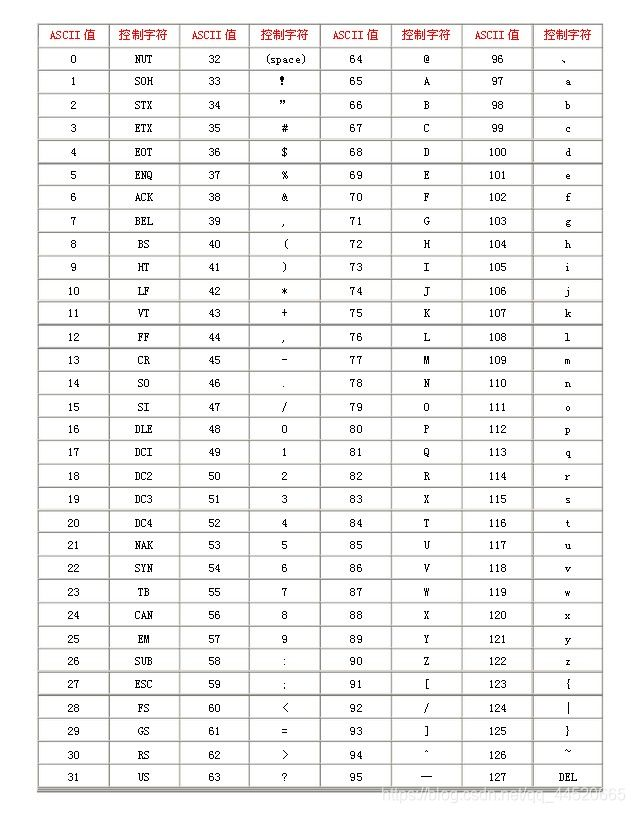
\includegraphics[width=0.9\linewidth]{pic/ascii.jpg}
        \caption{ASCII字符集对应表} \label{ASCII字符集对应表}
    \end{figure}

    \begin{table}[htbp]
        \centering
        \renewcommand\arraystretch{1.5}
        \begin{threeparttable}
            \begin{tabular}{|c|c|} 
                \hline
                ~数据类型~    & ~占用内存(B)~   \\
                \hline \hline
                int         & 4             \\
                \hline
                short       & 2             \\
                \hline
                long        & 4 或 8\tnote{1} \\
                \hline
                char        & 1             \\
                \hline
                float       & 4             \\
                \hline
                double      & 8             \\
                \hline
            \end{tabular} 
            \begin{tablenotes}
                \item[1] 因操作系统而异
            \end{tablenotes}
            \caption{数据类型占用内存表} \label{数据类型占用内存表}
        \end{threeparttable}
    \end{table} 

    \begin{table}[htbp]
        \centering
        \renewcommand\arraystretch{1.5}
        \begin{threeparttable}
            \begin{tabular}{|c|c|}
                \hline
                优先级  & 运算符\tnote{1} \\
                \hline \hline
                1       & \texttt{[]} \ \ \ \texttt{()} \ \ \ \texttt{.} \ \ \ \texttt{->} \\
                \hline
                \multirow{2}{*}{2}       & \texttt{-}$^{\mbox{\scriptsize 负号}}$ \ \ \ \texttt{+}$^{\mbox{\scriptsize 正号}}$ \ \ \ \texttt{(type)} \ \ \ \texttt{++} \ \ \ \texttt{--} \\  
                        & \texttt{*}$^{\mbox{\scriptsize 取值}}$ \ \ \ \texttt{\&}$^{\mbox{\scriptsize 取址}}$ \ \ \ \texttt{!} \ \ \ \texttt{$\sim$} \ \ \ \texttt{sizeof} \\
                \hline
                3       & \texttt{/} \ \ \ \texttt{*}$^{\mbox{\scriptsize 乘法}}$ \ \ \ \texttt{\%} \\
                \hline
                4       & \texttt{+}$^{\mbox{\scriptsize 加法}}$ \ \ \ \texttt{-}$^{\mbox{\scriptsize 减法}}$ \\
                \hline
                5       & \texttt{<<} \ \ \ \texttt{>>} \\
                \hline
                6       & \texttt{<} \ \ \ \texttt{>} \ \ \ \texttt{<=} \ \ \ \texttt{>=} \\
                \hline
                7       & \texttt{==} \ \ \ \texttt{!=} \\
                \hline
                8       & \texttt{\&}$^{\mbox{\scriptsize 按位与}}$ \\
                \hline
                9       & \texttt{\^{}} \\
                \hline
                10      & \texttt{|} \\
                \hline
                11      & \texttt{\&\&} \\
                \hline
                12      & \texttt{||} \\
                \hline
                13      & \texttt{?:} \\
                \hline
                \multirow{2}{*}{14}      & \texttt{=} \ \ \ \texttt{+=} \ \ \ \texttt{-=} \ \ \ \texttt{*=} \ \ \ \texttt{/=} \ \ \ \texttt{\%=} \\
                        & \texttt{<<=} \ \ \ \texttt{>>=} \ \ \ \texttt{\&=} \ \ \ \texttt{\^{}=} \ \ \ \texttt{|=} \\
                \hline
                15      & \texttt{,} \\
                \hline
            \end{tabular}
            \begin{tablenotes}
                \item[1] 表中运算符当发生歧义时运算符后用上标标注运算名称.
            \end{tablenotes}
            \caption{运算符优先级表} \label{运算符优先级表} 
        \end{threeparttable}
    \end{table}